\documentclass[12pt]{article}

\usepackage[margin=1.5cm]{geometry}
\usepackage{setspace, multicol, hyperref, graphicx, float, caption}

\singlespacing
\parindent=0pt
\parskip=6pt

\title{Pac-Man Algorithm Exploration}
\author{Dylan Ahearn, Aubrey Conners, Christopher Siems, Samuel Szymanski}
\date{2024 May 3}

\begin{document}
  \maketitle
  \section*{Abstract}
    This white paper discusses our exploration of mostly simple algorithms developed for playing Pac-Man. Winning a game of Pac-Man requires the player (in our case, the algorithms) to navigate through a maze collecting all dots (pacgums), while not losing all lives to the ghosts. On the surface, this sounds simple, but there is considerable complexity as you look deep. To explore this problem, we implemented a set of algorithms that take different approaches to finding paths through the mazes. Over the course of the past few month we explored 14 different algorithms based on a few ideas:
    \begin{multicols}{2}
      \begin{itemize}
        \itemsep0pt
        \item Randomness
        \item Breadth-first search (BFS)
        \item $A^*$
        \item Dijkstra's Algorithm
      \end{itemize}
    \end{multicols}
    We developed different Pac-Man algorithms based the ideas underpinning these well-known algorithms, with some of the more complex algorithms demonstrating aggression and inhuman efficiency. To enable these pathfinding algorithms we also developed a small suite of auxiliary helper algorithms that were capable of reuse in many parts of the code, such as point-to-point pathfinders for BFS, $A^*$, and Dijkstra's along with a parser algorithm capable of translating the level into a graph.
  \section*{Development}
    Development of this project began with the discovery and forking of an existing implementation of Pac-Man from GitHub, \href{https://github.com/usawa/pypacman}{usawa/pypacman}. We chose the path of forking existing code because building the base game, something that has already been done thousands of times, would be a time-consuming and unnecessary exercise in reinventing the wheel. Before any work could begin on development of our algorithms we first had to make some minor changes to the game's code so as to make it handle what it needed to.

    The next, and longest phase of development, was the production of the algorithms themselves. We began by creating a set of extremely basic algorithms based on simple randomness. These random algorithms served to help us familiarize ourselves with the structure of the project and provided a good comparison point for the more complex algorithms to come. Once we had assembled a good set of these simple algorithms we went on to develop the more complex ones.

    Once we were satisfied with our set of algorithms we wrote two simple scripts to benchmark each one. The first, runs each algorithm in sequence and collects data about that algorithm's performance, the data points collected include:
    \begin{itemize}
      \itemsep0pt
      \item Did the Pac-Man win?
      \item The number of pacgums collected.
      \item The score achieved.
    \end{itemize}
    The second script processes the dataset produced by the first into a set of charts enabling easy comparison of the performance of the algorithms.
  \section*{Algorithms}
    \begin{description}
      \itemsep0pt
      \item[Random Direction] This algorithm is by far the simplest. At each step of the game, this algorithm directs Pac-Man to face in a random direction.
      \item[Random Legal Direction] This algorithm is a slight modification of Random Direction. This algorithm works the same way, the only difference is that it will not choose to face in directions that Pac-Man cannot travel, e.g. it will not run Pac-Man into walls.
      \item[Random Hold Direction] This algorithm is another slight modification of Random Direction. This algorithm will pick a random direction and will continue in that direction until it cannot anymore, then it will pick a new direction.
      \item[Random Legal Hold Direction] This algorithm combines the two previous algorithms. This algorithm will only pick legal directions to move in and will only change directions when it has to.
      \item[Random Turn] This algorithm detects when Pac-Man is at a junction (a place in the level where Pac-Man can turn) and chooses a random direction for Pac-Man to move in.
      \item[Random Legal Turn] Like the previous algorithm and Random Legal Direction. This algorithm tells Pac-Man to move in a new direction only when he can and only tells Pac-Man to travel in directions with paths.
      \item[Random Charge] This algorithm directs Pac-Man to `charge' down a random walk through the level. Charge, in this case, means Pac-Man will pick a direction, move in that direction until he reaches a junction, and pick a new directions excluding the direction he came from.
      \item[BFS Random] This algorithm picks a random place in the level and uses BFS to find the optimal path through the level to that place. It repeats this process until the game is over.
      \item[BFS Pacgum] This algorithm performs BFS until it finds a place a pacgum. Once it finds a pacgum, it directs Pac-Man down the optimal path to that pacgum. This process is repeated until the game is over.
      \item[BFS Aggress] This algorithm prioritizes hunting the ghosts. Its process is to seek out, using BFS, one of the power-up pacgums (big-gums), then hunt down the nearest ghosts, using BFS, for as long as the power-up is active.
      \item[BFS Solver] This algorithm does not use the traditional BFS algorithm. It instead uses logic inspired by BFS to find the optimal path through all the pacgums in the level. In simplest terms, this algorithm queues up vertices to be checked, like BFS, but does not mark the vertices. This allows vertices to be revisited.
      \item[$A^*$ Random] This algorithm is the same as BFS Random but uses $A^*$ to pathfind with Manhattan distance as the heuristic.
      \item[$A^*$ Aggress] This algorithm is the same as BFS Aggress but uses the same version of $A^*$ as $A^*$ Random to pathfind.
      \item[Dijkstra Random] This algorithm is the same as BFS Random but uses Dijkstra's algorithm to pathfind.
    \end{description}
  \section*{Results}
    Of the algorithms we produced, only two of them were ever able to win a game of Pac-Man. This is not too surprising as we really did not set out with the goal of creating optimal Pac-Man playing systems, rather we just wanted to explore simple ideas for playing Pac-Man. The two algorithms were BFS Pacgum and BFS Solver, their associated win-rates are charted below in Figure 1.
    \begin{figure}[H]
      \begin{center}
        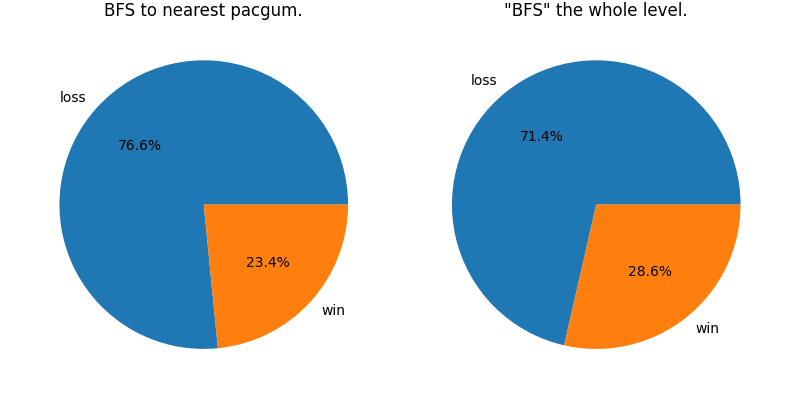
\includegraphics[width = .885\linewidth]{../../graphs/wins.png}
        \captionsetup{width = .885\linewidth}
        \caption{Pie charts depicting the win-rates of the two algorithms capable of winning, BFS Pacgum and BFS Solver.}
      \end{center}
    \end{figure}
    Both algorithms win at almost the same rates as each other. This makes intuitive sense as both algorithms are directly working to accomplish the same goal, they are just using different strategies. The code behind both algorithms seeks to collect pacgums, the main difference is BFS Pacgum seeks out only the nearest pacgum at each step and BFS Solver computes a path through each pacgum in the whole level before the game begins. Both algorithms prioritize collecting as many pacgums as they can as fast as they can and this similarity is reflected in the statistics. This similarity is also visible in the pacgum collection statistics. With both of these algorithms typically collecting a similar number of pacgums on any given game of Pac-Man. This property is visible in Figure 2 below.
    \begin{figure}[H]
      \begin{center}
        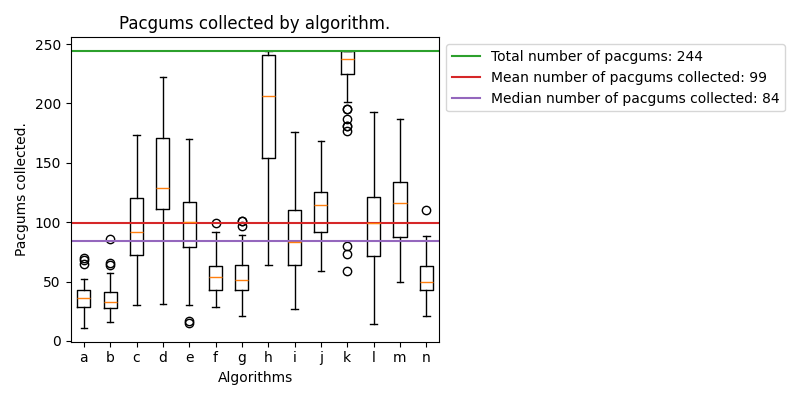
\includegraphics[width = .885\linewidth]{../../graphs/gums.png}
        \captionsetup{width = .885\linewidth}
        \caption{Box plot depicting the numbers of pacgums collected by each algorithm. For a key to reading the algorithm markers in this data, check the key section of this report.}
      \end{center}
    \end{figure}
    Algorithms $i$ and $k$ in Figure 2 are BFS Pacgum and BFS Solver respectively. The data shows exactly what we should expect knowing that these two algorithms win Pac-Man about a quarter of the time, that is, the upper edges of the bodies of their plots are in line with the number of pacgums needed to win. Another interesting detail elucidated by this chart is how good at Pac-Man Random Charge, algorithm $g$, is. From the description alone, one might think that Random Charge would be about as good at Pac-Man as the rest of the primarily random algorithms. But something we observed while testing this algorithm was that it plays in a manner that looks human, insofar as it plays confidently. On several occasions, we noticed this algorithm performing quite well, this is clearly reflected in the data. We think that given enough attempts, Random Charge would be able to win. Though in general it does seem that the complex `thinking' algorithms out perform the random algorithms. The main exception to this rule is Dijkstra Random, $n$, which scores about as well as the truly random algorithms. This is because Dijkstra Random is built from a faithful implementation of Dijkstra's Algorithm, which attempts to minimize the sum weight of the edges it traverses. When the weights signify the number of pacgums on a path, this creates an algorithm that deliberately avoids pacgums. While collecting pacgums is the required action for victory, Pac-Man is also independently scored. We tracked the scores received by our algorithms and these scores are shown in Figure 3 below.
    \begin{figure}[H]
      \begin{center}
        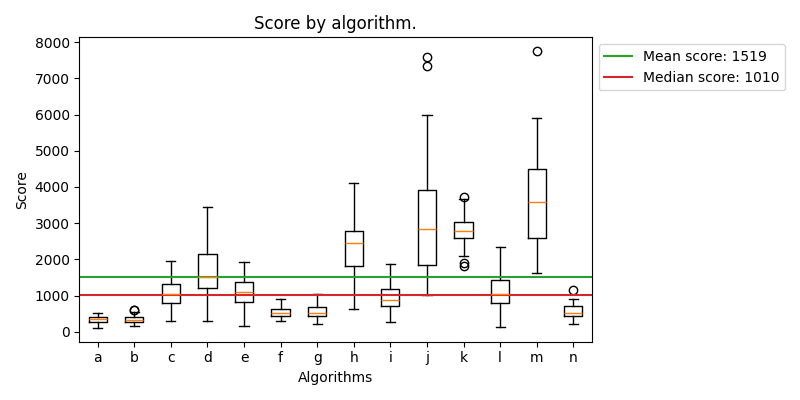
\includegraphics[width = .885\linewidth]{../../graphs/score.png}
        \captionsetup{width = .885\linewidth}
        \caption{Box plot depicting the scores received by each algorithm. For a key to reading the algorithm markers in this data, check the key section of this report.}
      \end{center}
    \end{figure}
    Interestingly, the winning algorithms, BFS Pacgum and BFS Solver ($i$ and $k$), are not particularly high scorers. This is the result of these algorithms' singular focus on collecting pacgums while ignoring the ghosts. Eating ghosts grants huge numbers of points, so it should not be shocking that the highest scoring algorithms are BFS Aggress, $j$, and $A^*$ Aggress, $m$. These algorithms score so much higher than the rest that this chart does not even include all of their data, some outliers had to be removed for the sake making the chart readable. The highest score achieved by any of our algorithms was 30,120, achieved by $A^*$ Aggress.

    Considering all of this data, there are two categories of `successful' algorithms. One category are the algorithms which successfully navigate the maze and collect all 244 pacgums thus winning. The other are the algorithms which scored much higher than the average score.  The algorithms which fit into the first category are BFS Pacgum and BFS Solver. However it should be noted that BFS Solver can take tens of minutes to compute its desired walk through the level, whereas BFS Pacgum does all computation in milliseconds. In practice, one is definitely better than the other. The other category contains the two algorithms that simulate aggressive behavior, BFS Aggress and $A^*$ Aggress. This strategy is unmatched in terms of score potential.
  \section*{Developer Guide}
    \begin{description}
      \itemsep0pt
      \item[Get the project] Go to \href{https://github.com/ChristopherSiems/PacmanAlgExploration}{ChristopherSiems/PacmanAlgExploration} on GitHub, fork the project, and clone your fork to your working device.
      \item[Install libraries] From within the project directory, run \texttt{pip install -r requirements.txt} in your command line to get the libraries you will need to run the project.
      \item[Make changes] Fix bugs, do optimization, add features, or write new algorithms all together. Before making any changes to existing files, be sure to consider how these changes will effect the other systems. If writing algorithms, be sure to include your algorithms in the \texttt{test.py} file so that data can be collected about their performance. As well, follow the shared structure of the algorithms:
        \begin{itemize}
          \itemsep0pt
          \item Create a new file in the \texttt{algs} folder which will contain your algorithm class.
          \item Create your algorithm as a Python class with a field \texttt{game} initialized to \texttt{None}, a method called \texttt{setup}, and a method called \texttt{get\_dir}.
          \item In \texttt{setup}, include any computation that should be done before the game begins. And in \texttt{get\_dir}, include the logic necessary to return the direction Pac-Man should travel in based on the game state.
          \item Import your algorithm into \texttt{pypacman.py}
        \end{itemize}
      \item[Collect data] Use \texttt{test.py} to collect data on the algorithms and use \texttt{graph.py} to generate new charts displaying the new performance. This may require erasing the current dataset if your changes are significant enough.
      \item[Open a pull request] If you want to see your changes included in the base project, open a pull request to ChristopherSiems/PacmanAlgExploration back on GitHub.
    \end{description}
  \section*{Milestones}
    We met the milestones we stated in the midterm report. We were able to successfully implement different pathfinding algorithms that control where Pac-Man moves into an automated Pac-Man game. We accomplished this despite the difficult process of developing and implementing the algorithms in an unfamiliar codebase.

    We were forced to pivot from some of the milestones that we stated in the initial report, as they proved to complex and time consuming to accomplish in a reasonable amount of time. Some things that we wanted to implement but were forced to drop include procedural generation of the levels, custom algorithms for the ghosts, more complex multi-state algorithms, and machine learning driven pathfinding. All of these are things that could be accomplished given enough time and work put into the project.
  \section*{Wish we had known.}
    As a group we came into this project lacking some of the important knowledge that we would go on to need in order to build some of the more complex algorithms. Not all of us started this semester with a great understanding of how some of the algorithms we would go on to use actually worked at the low level. This meant that implementing these algorithms were sometimes challenging, especially before we began the graphs section of this class.

    It would have definitely been useful to have come into this project knowing everything there is to know about $A^*$, Dijkstra's algorithm, graph representation, etc.. But unfortunately we did not all have perfect knowledge of these things and there is still, probably, a ton that we could learn. This lack of some necessary knowledge meant that development was slower than it could have been and that we probably accomplished less than we could have.
  \section*{Key}
    \begin{table}[H]
      \centering
      \begin{tabular}{c|c}
          Label & Algorithm\\
          \hline
          $a$ & Random Direction\\
          $b$ & Random Legal Direction\\
          $c$ & Random Hold Direction\\
          $d$ & Random Legal Hold Direction\\
          $e$ & Random Turn\\
          $f$ & Random Legal Turn\\
          $g$ & Random Charge\\
          $h$ & BFS Random\\
          $i$ & BFS Pacgum\\
          $j$ & BFS Aggress\\
          $k$ & BFS Solver\\
          $l$ & $A^*$ Random\\
          $m$ & $A^*$ Aggress\\
          $n$ & Dijkstra Random
      \end{tabular}
      \caption{Mapping of chart algorithm labels to algorithms}
    \end{table}
  \vfill
  Typeset with \LaTeX.
\end{document}